\documentclass[a4paper, 12pt]{article}
\usepackage{titling}
\usepackage{array}
\usepackage{booktabs}
\usepackage{enumitem}
\usepackage{graphicx}
\usepackage{hyperref}
\usepackage{amssymb}
%\usepackage{mathtools}
\usepackage{listings}
\usepackage{amsmath}
\usepackage{color} %red, green, blue, yellow, cyan, magenta, black, white
\setlength{\heavyrulewidth}{1.5pt}
\setlength{\abovetopsep}{4pt}
\setlength{\parindent}{0pt}
\graphicspath{{.}}
\usepackage{float}
\usepackage[margin=1in]{geometry}
\definecolor{mygreen}{RGB}{28,172,0} % color values Red, Green, Blue
\definecolor{mylilas}{RGB}{170,55,241}
% Must be after geometry
\usepackage{fancyhdr}
\pagestyle{fancy}
\fancyhf{}
\rhead{NN Homework 9}
\lhead{P.Lukin, E. Ovchinnikova}
\cfoot{\thepage}

\setlength{\droptitle}{-5em}

\title{Neural Networks  \\
				- Homework 9 -}
\author{Petr Lukin, Evgeniya Ovchinnikova}
\date{Lecture date: 21 November 2016}

\begin{document}

%-------------------------------------------------------------------------------
\lstset{language=Matlab,%
    %basicstyle=\color{red},
    breaklines=true,%
    morekeywords={matlab2tikz},
    keywordstyle=\color{blue},%
    morekeywords=[2]{1}, keywordstyle=[2]{\color{black}},
    identifierstyle=\color{black},%
    stringstyle=\color{mylilas},
    commentstyle=\color{mygreen},%
    showstringspaces=false,%without this there will be a symbol in the places where there is a space
    numbers=left,%
    numberstyle={\tiny \color{black}},% size of the numbers
    numbersep=9pt, % this defines how far the numbers are from the text
    emph=[1]{break},emphstyle=[1]\color{red}, %some words to emphasise
    emph=[2]{end,function}, emphstyle=[1]\color{blue},
}

%-------------------------------------------------------------------------------

\maketitle

\section{Mind map}
\begin{figure}[h]
  \centering
  \caption{Mind map. Chapter 9 from Haykin's book. A zoomed version is attached as SOMs.png}
  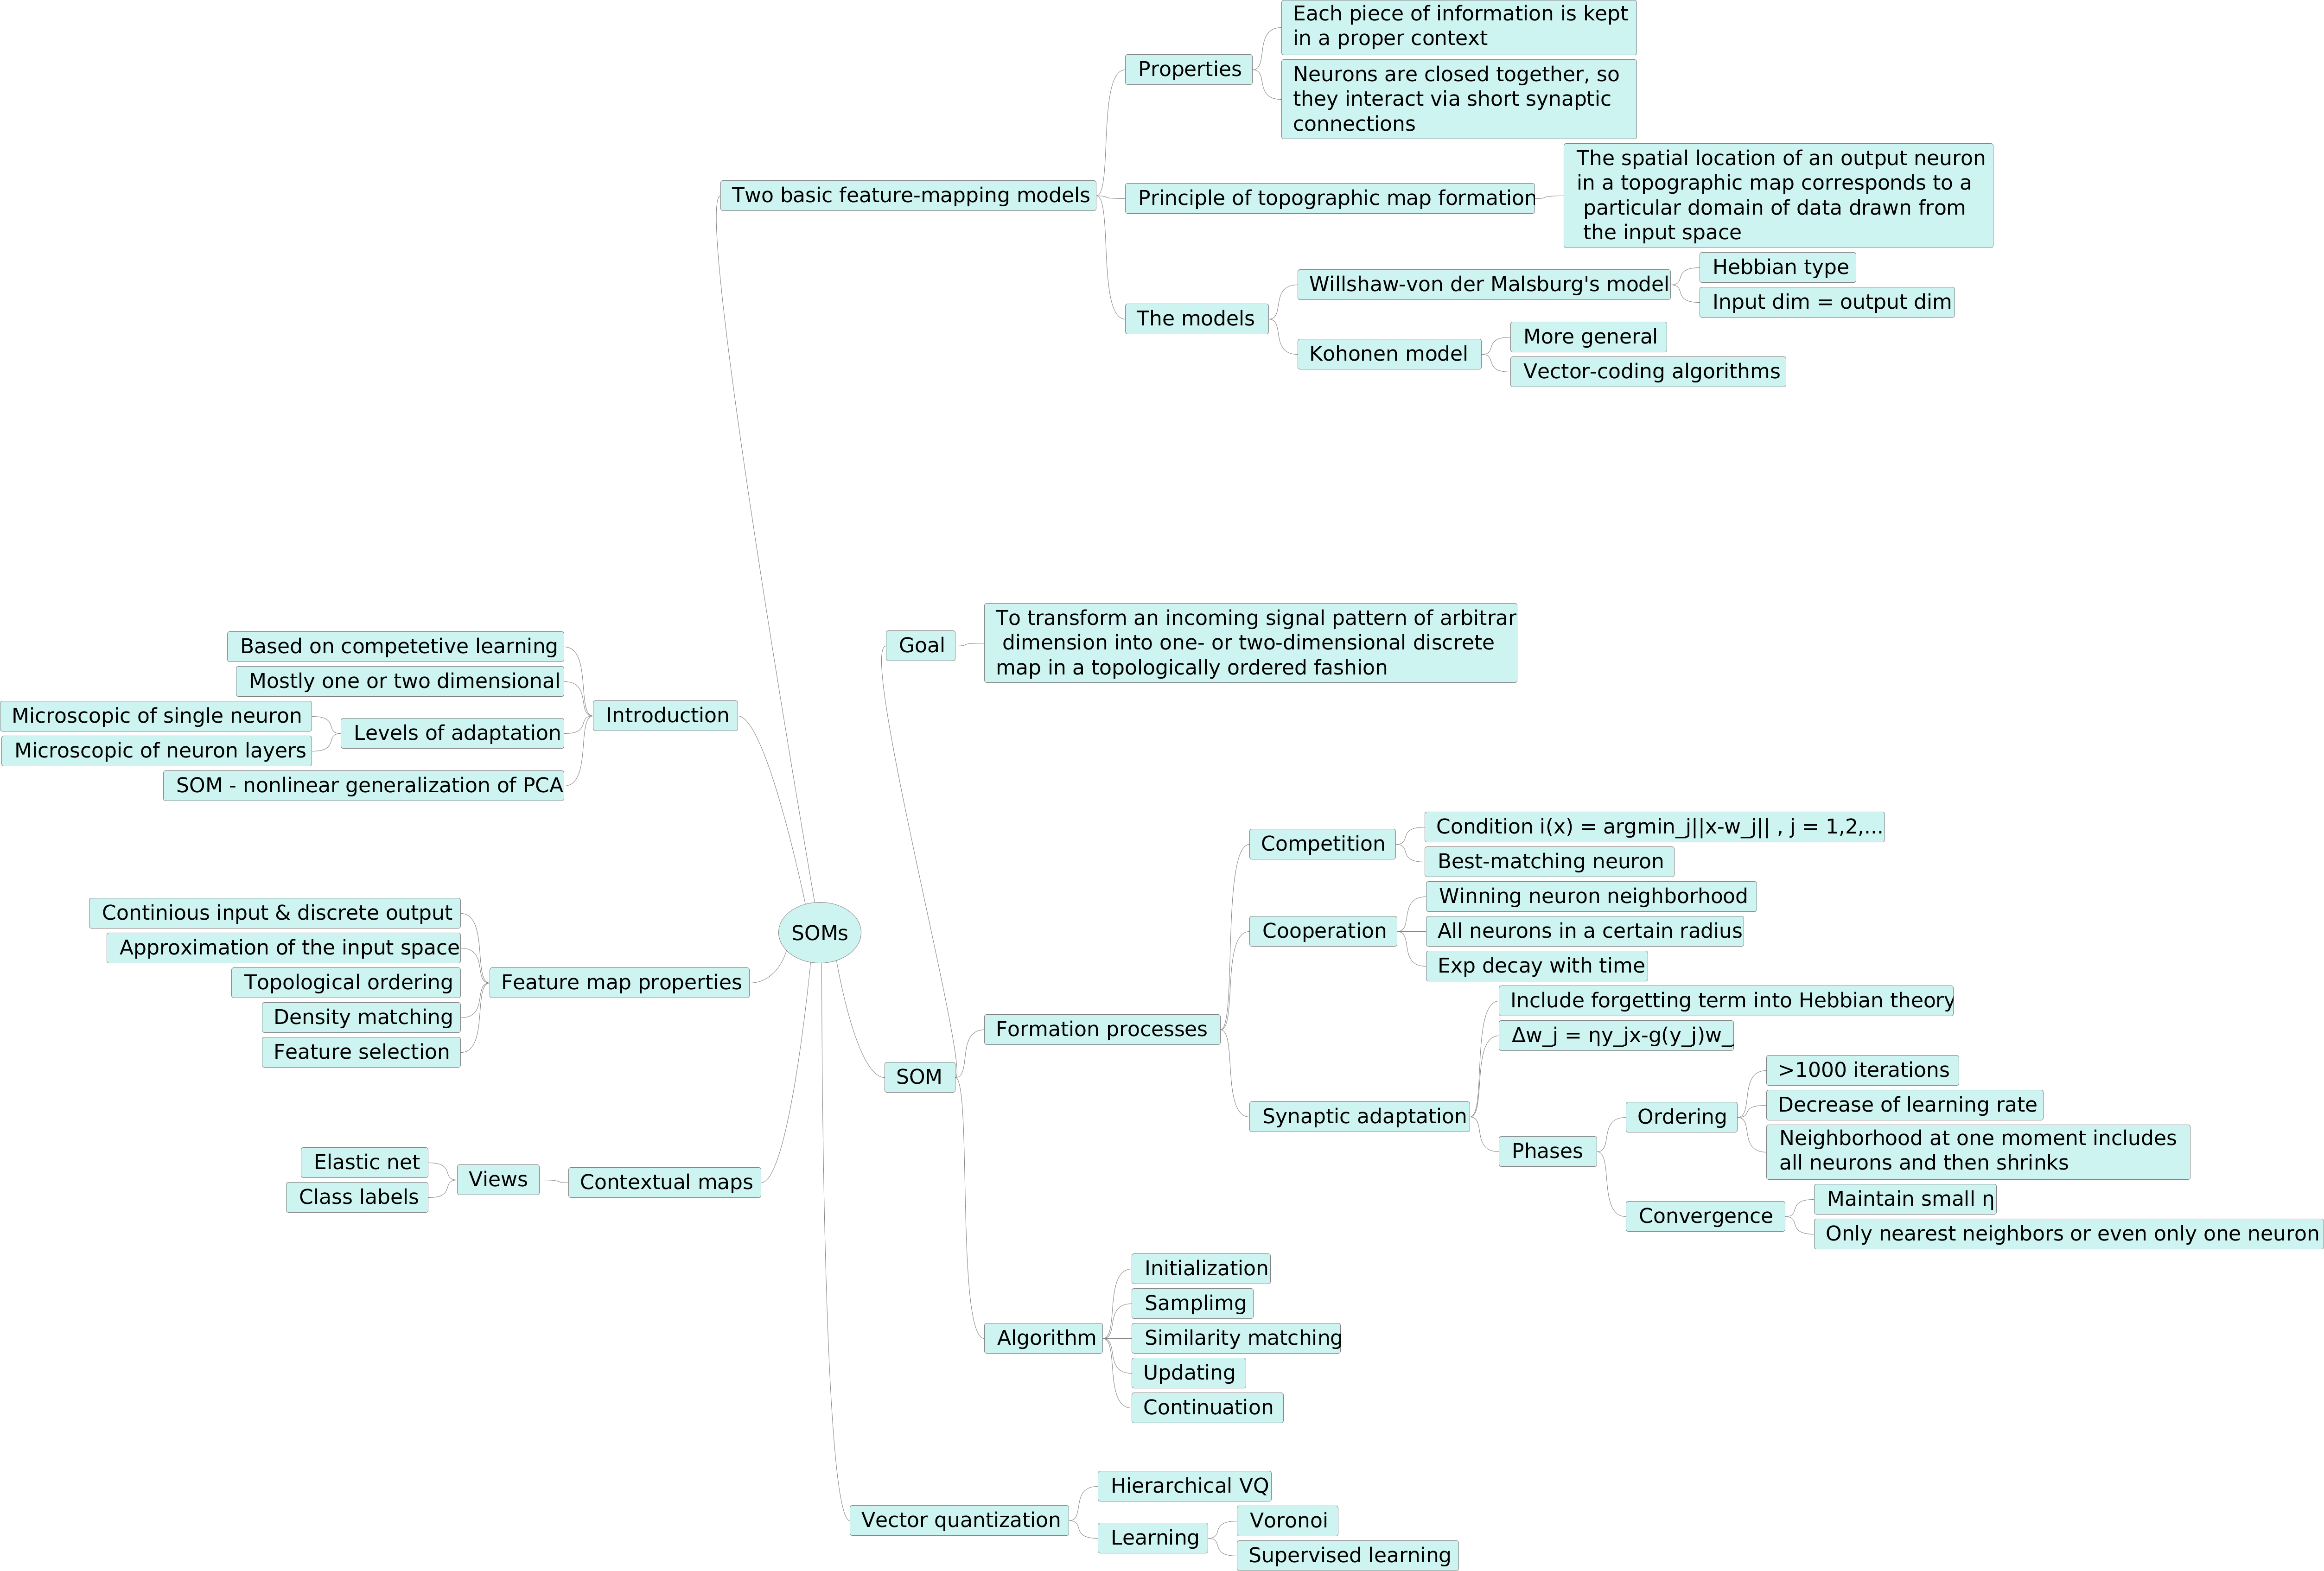
\includegraphics[width=1.0\textwidth]{SOMs}
\end{figure}

\newpage
\section{Exercises}

\subsection{Exercise 2}
Show that in the SOM algorithm the winner neuron for an input $x$ is the neuron $k$ whose weight vector $w_k$ maximizes the inner product $< w k ,x >$ of x and w k , with $x$ and $w_k$ normalized.


The closest neuron will satisfy the following condition:

\begin{equation}
k(x) = arg \min\limits_k \parallel x-w_k \parallel^2,
\end{equation}
where $k$ - index of winning neuron, $x$ - current input signal. Let's rewrite this equation:

\begin{equation}
\min\limits_k \parallel x-w_k \parallel^2 = \min\limits_k (x-w_k)*(x^T-w_k^T) =  \min\limits_k x x^T-w_k x^T - x w_k^T + w_k w_k^T = \min\limits_k x x^T - 2  w_k x^T + w_k w_k^T.
\end{equation}

Because $min$ function does not depend on $x$ and $w_k$ is normalized, we can omit some terms:

\begin{equation}
\min\limits_k \parallel x-w_k \parallel^2 =\min\limits_k  - 2 w_k x^T + 1 = \min\limits_k  - 2 w_k x^T = \max\limits_k 2 w_k x^T = \max\limits_k w_k x^T.
\end{equation}

Thus, winner neuron maximizes inner product $<w_k,x>$.
\subsection{Exercise 3}

Consider the one dimensional input space S={0.1, 0.2, 0.4, 0.5}.
Cluster S using a one dimensional SOM network with:

\begin{itemize}
\item 2 nodes.
\item learning rate equal to 0.1.
\item Neighborhood function which is equal to 1 for the winner neuron and is 0 otherwise.
\item Weight initialization:
\begin{itemize}
\item $w_1$=0.15, $w_2$=0.45
\item $w_1$=0.3, $w_2$=0.9
\end{itemize}
\item Stopping criterion: $$\sum_{i=1}^2|w_i^{old} - w_i^{new}| < 0.01$$
\end{itemize}

Comment on the two clusterings you obtained using the two different weight initializations.

\bigskip
\newpage
Solution to this problem is not deterministic. Due to fixed learning rate, neurons will react each time we input data. However, stop criterion is too weak and convergence can be achieved in 2 iteration. So, the neurons will oscillate around the initial weights.

\begin{figure}[h]
  \centering
  \caption{Typical weight distribution with initialization $[0.15, 0.45]$.}
  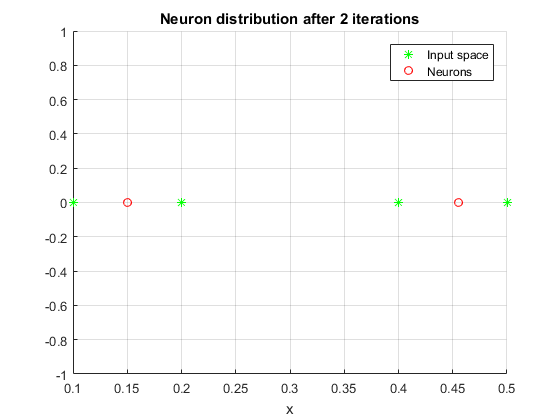
\includegraphics[scale = 0.7]{1}
\end{figure}

In the second case: $[0.3, 0.9]$, the first neuron will be always a winner, given this input space. And this neuron will oscillate oscillate around initial value.

\begin{figure}[h]
  \centering
  \caption{Typical weight distribution with initialization $[0.3, 0.9]$.}
  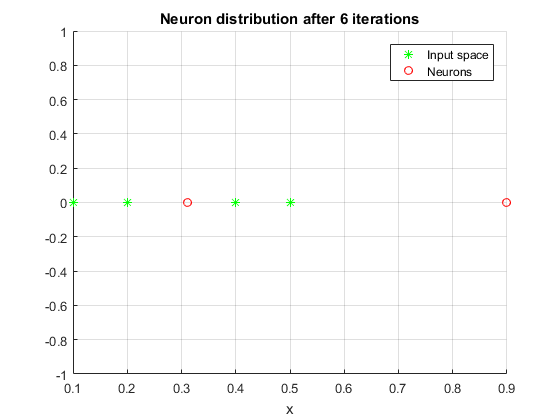
\includegraphics[scale = 0.7]{4}
\end{figure}

 \clearpage
 If we strengthen the criterion $$\sum_{i=1}^2|w_i^{old} - w_i^{new}| < 0.001$$ random nature of the solution will be clearly seen.

 \begin{figure}[h]
  \centering
  \caption{Typical weight distribution with initialization $[0.15, 0.45]$ and $\nu = 0.001$.}
  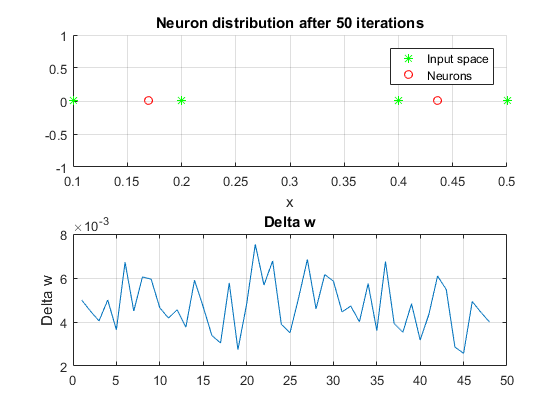
\includegraphics[scale = 0.7]{2}
\end{figure}
We can partially avoid this oscillations by adding learning rate decay. For example, we can use this rule: $\nu(k) = nu_0 \exp^{-k/2}$.
\begin{figure}[h]
  \centering
  \caption{Weight distribution with initialization $[0.15, 0.45]$ and $\nu$ decay.}
  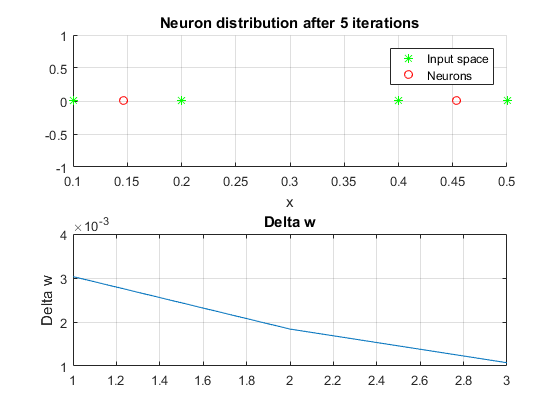
\includegraphics[scale = 0.7]{3}
\end{figure}

 \clearpage
Finally, if we conduct multiple experiment with the same initial weights, mean value of weights will be the initial ones.

\begin{figure}[h]
  \centering
  \caption{Mean of distribution with initialization $[0.15, 0.45]$ and $\nu$ decay.}
  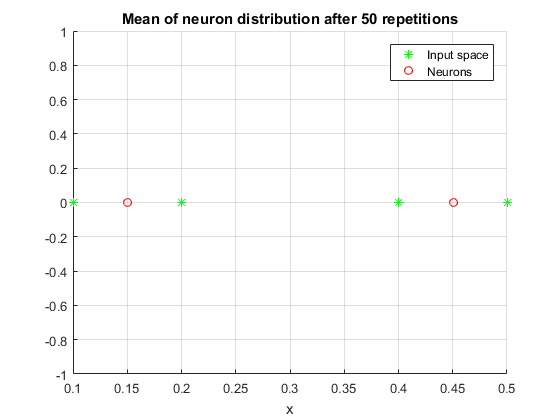
\includegraphics[scale = 0.7]{1mean}
\end{figure}

\begin{figure}[h]
  \centering
  \caption{Mean of distribution with initialization $[0.3, 0.9]$ and $\nu$ decay.}
  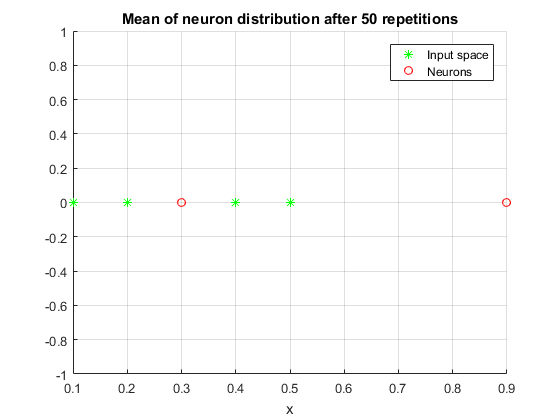
\includegraphics[scale = 0.7]{2mean}
\end{figure}

\newpage 
\subsection{Exercise 4}
Program a SOM to solve the traveling salesman problem (TSP):
\begin{itemize}
\item  Input layer contains just two neurons called "Xcoord" and "Ycoord"
\item The Kohonen lattice is thought of as a circle containing at least as many neurons as we have cities (usage of more neurons is possible), the neurons are numbered in round about fashion.
\item Each neuron n(i) (numbered by i) on the circle is connected to "Xcoord" and "Ycoord" and the weights on these edges are the initial x and y coordinates of the neuron in the plane (see picture)
\item The input patterns are the (x,y) coordinates of all target cities.
\item When applying one concrete city pattern the winner is of course the neuron with lies closest to the given city. Only the weights of the winning neuron will be adapted according to the learning rule, no other neighboring weights are changed. This "moves" the neuron closer to "its" city.
\item After some cycles there is just ONE neuron closest to each city. These build pairs (n(i),City(closest to n(i)).
\item If we sort this pairs according to the number of the neurons "i" this will give a journey for the respective cities, which solves the TSP approximately.
\item Use tools like ICONNECT, TSPLIB or alike to do the programming, compare runtime, memory and achieved length of path.
\end{itemize}

\begin{figure}[h]
  \centering
  \caption{Cities for TSP.\label{cities}}
  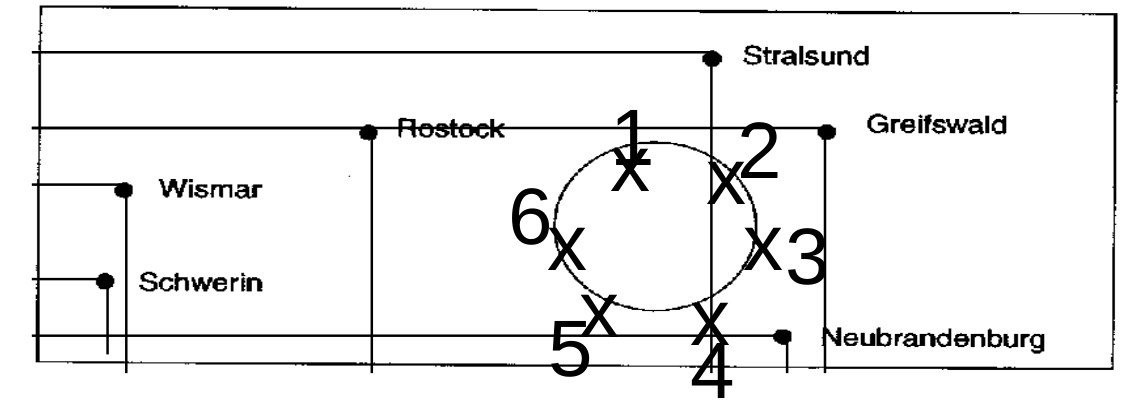
\includegraphics[width=0.5\textwidth]{cities}
\end{figure}


Solution:\\

First we plot the cities and randomly initialized on a circle of radius 3 initial neuron weights (Fig. \ref{citiesCoord}). One can see that here we have 12 -more than 6 hidden neurons. The reason is that with 6 and even 10 neurons we ended up in a local minimum - with one neuron stuck between two cities. It is also important that we are sorting the neurons coordinates by angle in polar coordinates so they would be enumerated from 1 to 12 in a circle.

\begin{figure}[h]
  \centering
  \caption{Cities on coordinate plane.\label{citiesCoord}}
  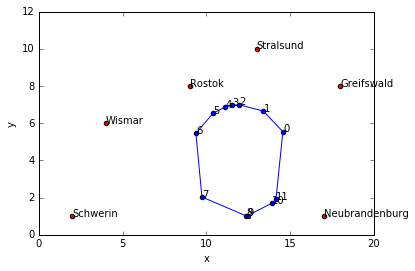
\includegraphics[width=0.5\textwidth]{cities_plotted}
\end{figure}

To initialize the weight and create those points we used the following code:

\lstset{language=Python}
\begin{lstlisting}[frame=single]
import numpy as np
import matplotlib.pyplot as plt
import math
from numpy import linalg as LA
%matplotlib inline

cities_names = np.array([ "Wismar", "Rostok", "Stralsund", "Schwerin","Greifswald", "Neubrandenburg"])
cities_coordinates = np.array([[4,6],[9,8],[13,10],[2,1],[18,8],[17,1]])

leng = 12
neuron_numbers = np.arange(leng)

angles = np.random.randint(0, 360, leng)
angles = angles*math.pi/180
angles = np.sort(angles)
print angles

r = 3
circle_x = np.array([])
circle_y = np.array([])

for angle in angles:
    x = r*math.cos(angle) + 12
    y = r*math.sin(angle) + 4
    circle_x = np.append(circle_x, x)
    circle_y = np.append(circle_y, y)

initial_weights = np.column_stack((circle_x, circle_y))
weights = initial_weights

def plot(cities_coordinates, weights):
    fig, ax = plt.subplots()
    ax.scatter(cities_coordinates[:,0], cities_coordinates[:,1], c = 'r')
    ax.scatter(weights[:,0], weights[:,1], c = 'b')

    #ax.annotate(cities_names[0], xy=cities_coordinates[], xytext=(3, 1.5))

    for i in range(len(cities_names)):
        ax.annotate(cities_names[i], (cities_coordinates[i,0],cities_coordinates[i,1]))
    for i in range(len(neuron_numbers)):
        ax.annotate(neuron_numbers[i], (weights[i,0],weights[i,1]))
    plt.plot(np.append(weights[:,0], weights[0,0]), np.append(weights[:,1], weights[0,1]))
    plt.show()

plot(cities_coordinates, weights)
\end{lstlisting}

Next part of the program implements the learning. In a cycle over all cities we check the distances between the city and neurons and move the closest neuron to the city according to the following formula:

$w_j(n+1) = w_j(n) _ \eta(n) h_{j,i(x)}(n)(x(n) - w_j(n))$,
where $\eta$ is a learning rate, $h_{j,i(x)}$ is a neighboring function, which is not really important in our case since we are required to use only one neuron, and x - coordinates of a city of our concern. We repeat it until the overall distance between cities and neurons is less than 0.0001.


\lstset{language=Python}
\begin{lstlisting}[frame=single]
change = 100
step = 0
summ = 100
indices = np.array([])

while(abs(summ) > 0.0001):
    summ = 0
    indices = np.array([])
    for city in cities_coordinates:
        #Determine the winning neuron
        dists = np.array([])
        for weight in weights:
            dist = math.hypot(city[0]-weight[0], city[1]-weight[1])
            dists = np.append(dists, dist)
        winner_index = np.argmin(dists)
        indices = np.append(indices, winner_index)
        #Adapt the weights of the winner neuron:
        weights[winner_index] = weights[winner_index] + eta(step)*(city - weights[winner_index])
        change = LA.norm(eta(step)*(city - weights[winner_index]))
        summ += change
    step += 1
print step
indices = np.sort(indices)
print indices

>> 224
>> [  0.   4.   5.   6.   8.  11.]
\end{lstlisting}

The algorithm converged in 224 steps and returned us the indices of neurons those are the closest to the cities. In order to find an optimal way we need to sort them. So, now we can plot the neurons with the cities and a path (Fig.\ref{fig:path}). The path length = 42.6951.

\begin{figure}[!htb]
\minipage{0.5\textwidth}
  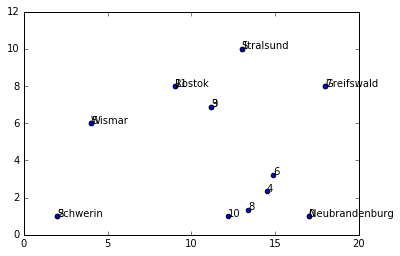
\includegraphics[width=\linewidth]{neuronsWithCities}
  \caption{Final neurons' positions.}\label{fig:neuronsWithCities}
\endminipage\hfill
\minipage{0.5\textwidth}
  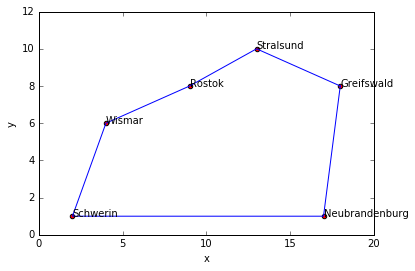
\includegraphics[width=\linewidth]{path}
  \caption{Path.}\label{fig:path}
\endminipage\hfill
\end{figure}

For that we used the following code:

\lstset{language=Python}
\begin{lstlisting}[frame=single]
#drop not needed weights
weights_assigned = weights[indices[0]]
for i in range(1,6):
    weights_assigned = np.row_stack((weights_assigned, weights[indices[i]]))
weights_assigned = np.row_stack((weights_assigned, weights[indices[0]]))

fig, ax = plt.subplots()
ax.scatter(cities_coordinates[:,0], cities_coordinates[:,1], c = 'r')

#ax.annotate(cities_names[0], xy=cities_coordinates[], xytext=(3, 1.5))

length = 0
for i in range(len(cities_names)):
    ax.annotate(cities_names[i], (cities_coordinates[i,0],cities_coordinates[i,1]))
    length += math.hypot(weights_assigned[i,0]-weights_assigned[i+1,0], weights_assigned[i,1]-weights_assigned[i+1,1])

plt.plot(weights_assigned[:,0], weights_assigned[:,1])
plt.show()
print length

>>42.6951103552
\end{lstlisting}

In the end we need to compare our solution with the one that will be returned by Concorde TSPLIB (Fig. \ref{pathConcorde}). The paths are identical. It is hard to estimate time and memory, because in both cases they are too small. Concorde rounded time to 0.

\begin{figure}[h]
  \centering
  \caption{TSPLIB path.\label{pathConcorde}}
  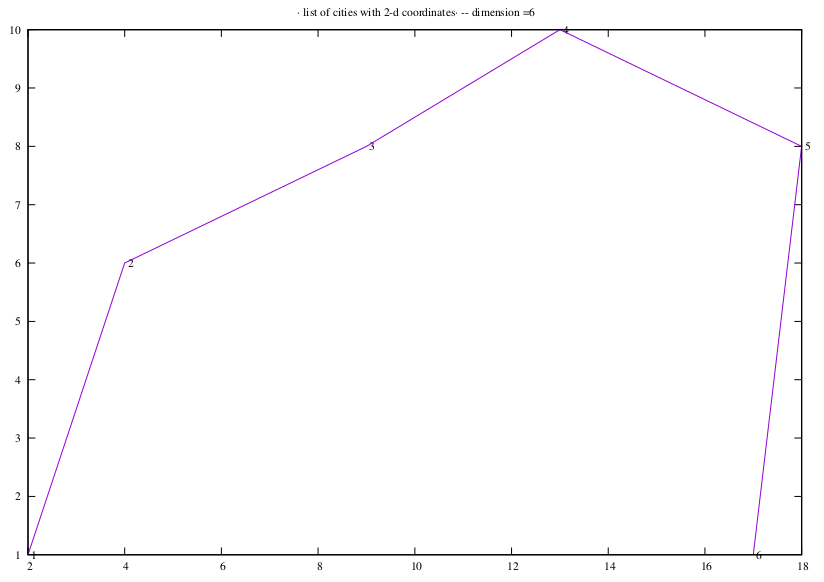
\includegraphics[width=0.5\textwidth]{pathConcorde}
\end{figure}

\end{document}
